\documentclass[tikz,border=10pt]{standalone}
\usepackage{tikz}
\usetikzlibrary{arrows.meta, positioning, fadings, shapes.arrows}

\begin{document}
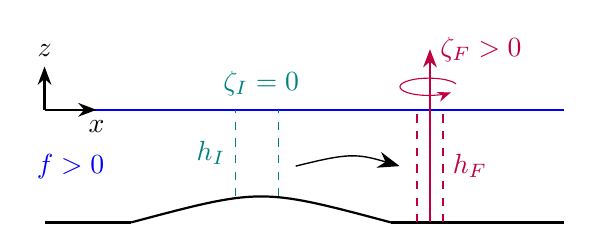
\begin{tikzpicture}[scale=1.1, >=Stealth]

    \draw[thick, black] (1,0) .. controls (2.5,0.4) .. (4,0);
    \draw[thick, black] (4,0) -- (6,0);
    \draw[thick, black] (0,0) -- (1,0);

    \draw[thick, blue] (0,1.3) -- (6,1.3);

    % put a label above this that says f>0:
    \node[text=blue] at (0.3,1.3/2) {$f > 0$};

    \draw[dashed, teal] (2.2, 0.3) -- (2.2,1.3) node[midway, left] {$h_I$};
    \draw[dashed, teal] (2.7, 0.3) -- (2.7,1.3);
    % put a label above this that says \zeta_I = 0:
    \node[text=teal] at (2.5,1.6) {$\zeta_I = 0$};

    \draw[dashed, purple] (4.3, 0) -- (4.3,1.3);
    \draw[dashed, purple] (4.6, 0) -- (4.6,1.3) node[midway, right] {$h_F$};

    \draw[->, thick, purple] (4.45, 0) -- (4.45, 2.) node[right] {$\zeta_F>0$};
    \begin{scope}[shift={(4.45,1.6,0)}]
        \draw[->, purple] (0.3,0) arc[start angle=20, end angle=320, x radius=1/3, y radius=0.3/3];
    \end{scope}

    % draw a squiggly arrow from 2.7 to 4.3 at 1.3/2
    \draw[thick, black, -{Stealth[scale=1.5]}, line width=0.5pt] (2.9,0.65) .. controls (3.5,0.8) and (3.6,0.8) .. (4.1,0.65) ;

    % small axes indicating x and y directions:
    \draw[->, thick] (-0,1.3) -- (0.6,1.3) node[below] {$x$};
    \draw[->, thick] (-0,1.3) -- (-0,1.8) node[above] {$z$};

%
\end{tikzpicture}
\end{document}
